\documentclass{beamer}
\usepackage[utf8]{inputenc}

\usetheme{Madrid}
\usecolortheme{default}
\usepackage{amsmath,amssymb,amsfonts,amsthm}
\usepackage{txfonts}
\usepackage{multicol}
\usepackage{tkz-euclide}
\usepackage{listings}
\usepackage{adjustbox}
\usepackage{array}
\usepackage{tabularx}
\usepackage{gvv}
\usepackage{lmodern}
\usepackage{circuitikz}
\usepackage{tikz}
\usepackage{graphicx}
\usepackage{hyperref}
\usepackage{siunitx}

\setbeamertemplate{page number in head/foot}[totalframenumber]

\usepackage{tcolorbox}
\tcbuselibrary{minted,breakable,xparse,skins}



\definecolor{bg}{gray}{0.95}
\DeclareTCBListing{mintedbox}{O{}m!O{}}{%
  breakable=true,
  listing engine=minted,
  listing only,
  minted language=#2,
  minted style=default,
  minted options={%
    linenos,
    gobble=0,
    breaklines=true,
    breakafter=,,
    fontsize=\small,
    numbersep=8pt,
    #1},
  boxsep=0pt,
  left skip=0pt,
  right skip=0pt,
  left=25pt,
  right=0pt,
  top=3pt,
  bottom=3pt,
  arc=5pt,
  leftrule=0pt,
  rightrule=0pt,
  bottomrule=2pt,
  toprule=2pt,
  colback=bg,
  colframe=orange!70,
  enhanced,
  overlay={%
    \begin{tcbclipinterior}
    \fill[orange!20!white] (frame.south west) rectangle ([xshift=20pt]frame.north west);
    \end{tcbclipinterior}},
  #3,
}
\lstset{
    language=C,
    basicstyle=\ttfamily\small,
    keywordstyle=\color{blue},
    stringstyle=\color{orange},
    commentstyle=\color{green!60!black},
    numbers=left,
    numberstyle=\tiny\color{gray},
    breaklines=true,
    showstringspaces=false,
}
%------------------------------------------------------------
%This block of code defines the information to appear in the
%Title page
\title %optional
{12.18}
\date{October 9,2025}
%\subtitle{A short story}

\author % (optional)
{Aditya Appana - EE25BTECH11004}

\begin{document}


\frame{\titlepage}
\begin{frame}{Question}
The $S_2$ operation on a molecule with the axis of rotation as the Z-axis, moves a nucleus at $(x,y,z)$ to
\begin{enumerate}
\begin{multicols}{4}
    \item $(-x,-y,z)$
    \item $(x,-y,-z)$
    \item $(-x,y,-z)$
    \item $(-x,-y,-z)$
\end{multicols}
\end{enumerate}
\end{frame}



\begin{frame}[fragile]
    \frametitle{Solution}
The rotation matrix for a rotation by an angle $\theta$ about the z-axis is:
\begin{align}
R_z(\theta) = \myvec{
\cos\theta & -\sin\theta & 0 \\
\sin\theta & \cos\theta & 0 \\
0 & 0 & 1}
\end{align}\\
Let the point be $\vec{x} = \myvec{x\\y\\z}$. Therefore the rotated vector will be:
\begin{align}
 R_z(\theta)\vec{x} =
 \myvec{\cos\theta & -\sin\theta & 0 \\\sin\theta & \cos\theta & 0 \\0 & 0 & 1}\myvec{x\\y\\z}\\
 \myvec{x\cos\theta - y\sin\theta \\ x\sin\theta +y\cos\theta \\ z}
\end{align}\\

\end{frame}
\begin{frame}[fragile]
    \frametitle{Solution}
It can be seen that a rotation about the Z-axis does not change the z-coordinate. Hence option (\textbf{A}) is correct.
\end{frame}


\begin{frame}[fragile]
    \frametitle{Code}
\href{https://github.com/AdityaAppana/ee1030-2025/tree/7296aff407ab736741f448272403a443c5153f2e/ee25btech11004/matgeo/12.122/Codes}{Codes Permalink}
\end{frame}

\begin{frame}[fragile]
    \frametitle{Figure}
\begin{figure}[H]
    \centering
    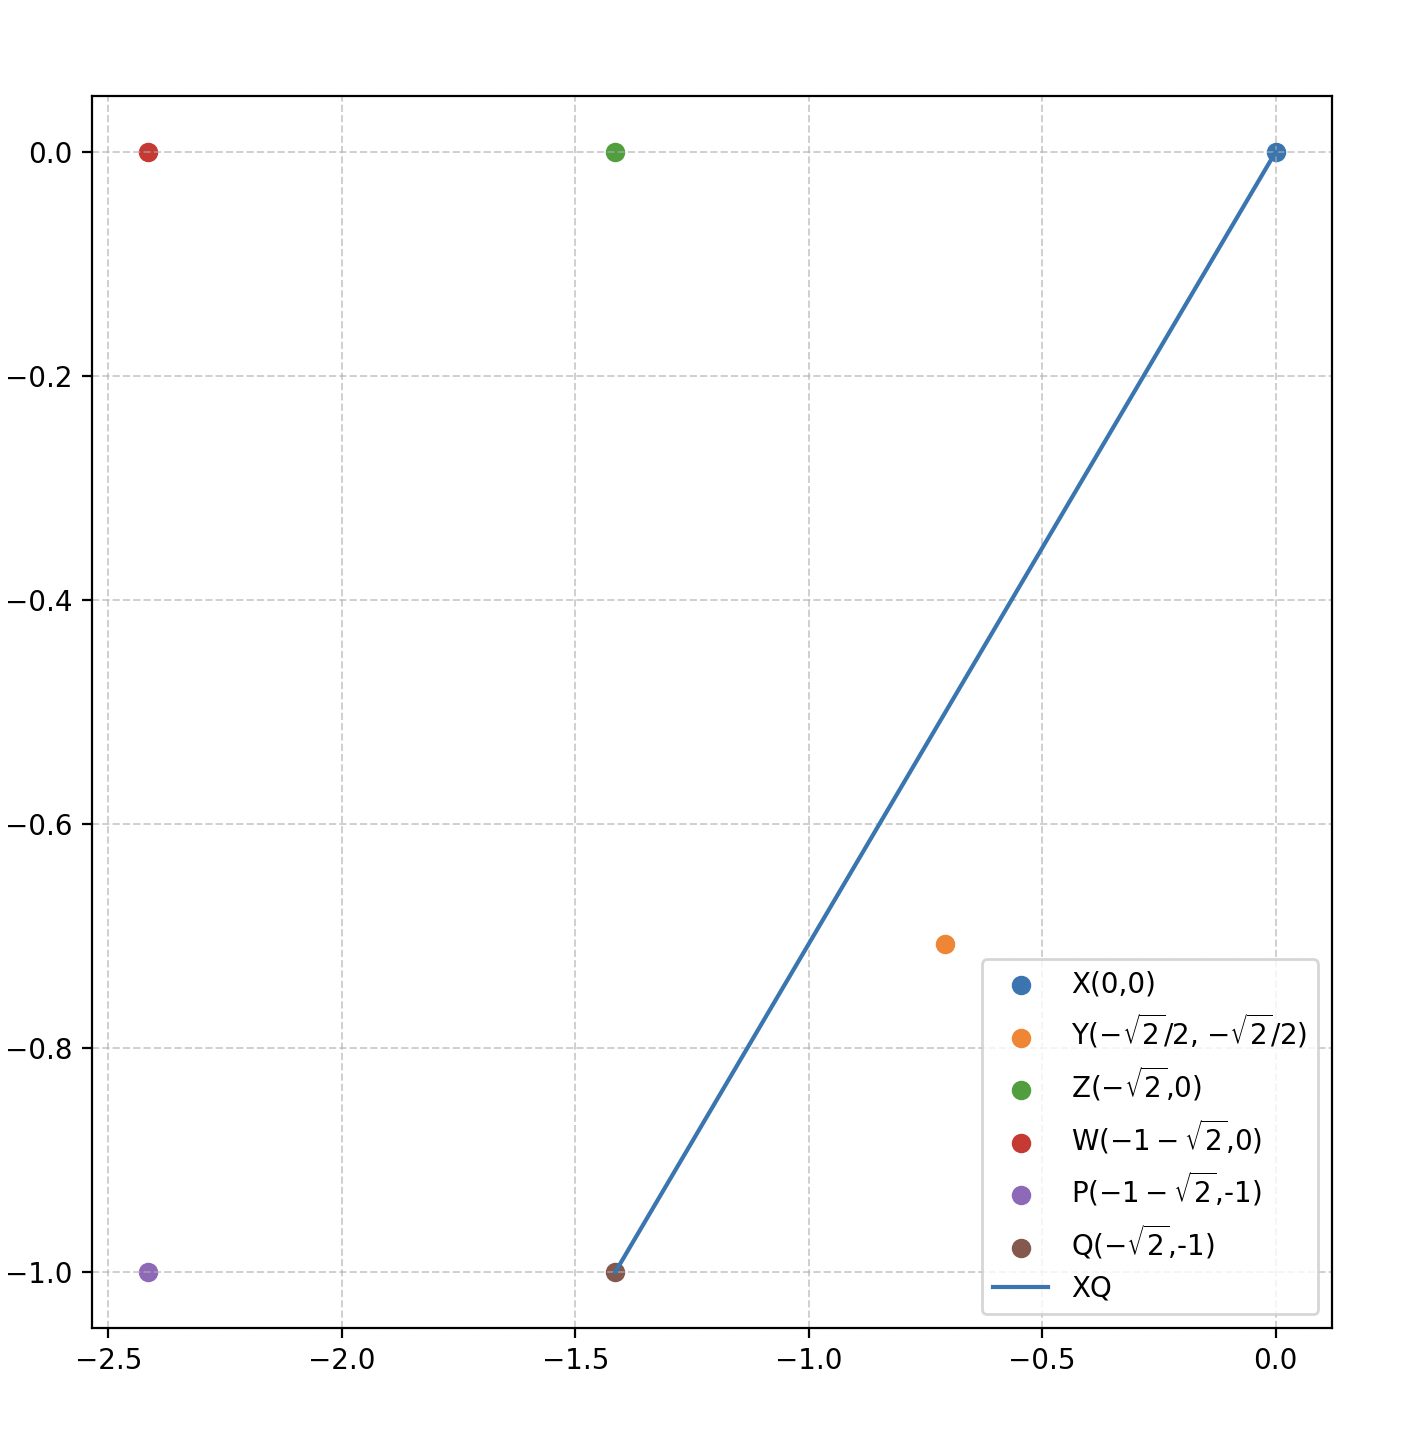
\includegraphics[width=0.6\columnwidth]{Figs/1218.png}
    \caption{Plot}
    \label{fig:placeholder}
\end{figure}
\end{frame}

\end{document}